\chapter{Hardware}
\section{Hardware Designs}
\subsection{ASIC - Application Specific Integrated Circuit}

\subsection{FPGA - Field-Programmable Gate Array}
In comparison to ASICs the FPGA can be programmed for different applications after delivery. The programming is done by combining a large number of logic blocks (CLB, LAB) and lookup tables (LUTs) through configurable bus connections. As FPGAs are reprogrammable, a design change in very late design phases is possible, even over remote connections. A general structure of a FPGA can be seen in figure \ref{fig:fpgablocksgeneral}. A FPGA is programmed using a HDL (see section \ref{kap:HDL}).
\begin{figure}[htbp]
\begin{center}
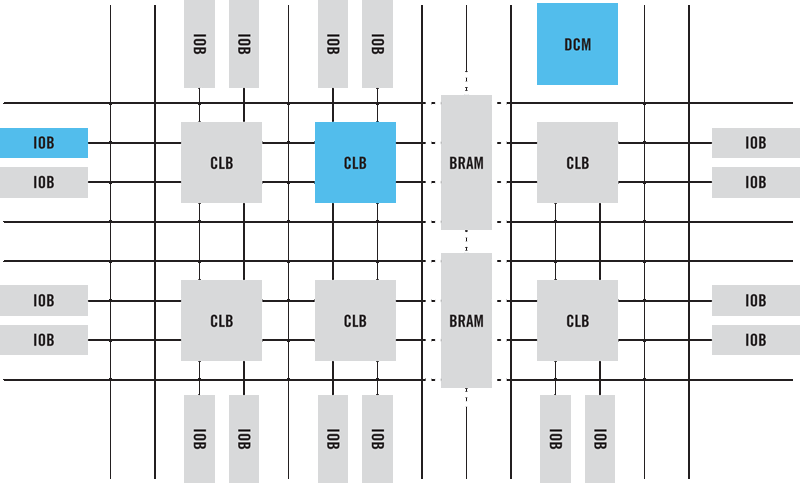
\includegraphics[width=14cm,keepaspectratio=true]{bilder/png/fpgablocksgeneral}
\caption{Internal design of FPGAs}
\label{fig:fpgablocksgeneral}
\end{center}
\end{figure}
\subsubsection{logic blocks}

\subsubsection{Look-up tables}
\subsubsection{SRAM-based devices}
The most common FPGA type is SRAM-based. SRAM cells are typically made of 4 to 6 MOSFET transistors (but also special factoring types with up to 10 transistors exist). The transistors are connected as bistable flipflops to store each bit. A typical SRAM cell is shown in figure \ref{fig:SRAMaufbau}. So those devices are volatile and have to be programmed each time they are powered up. As they can be programmed further and further again they are suitable for prototyping and updating the configuration. As disadvantages it has to be mentioned that SRAM-based devices are more sensitive to radiation and therefore they need additional shielding. Furthermore, due to the physical design they need more space and so less space for logic arrays is available.\cite{Maxfield2009}\\
\begin{figure}[htbp]
\begin{center}
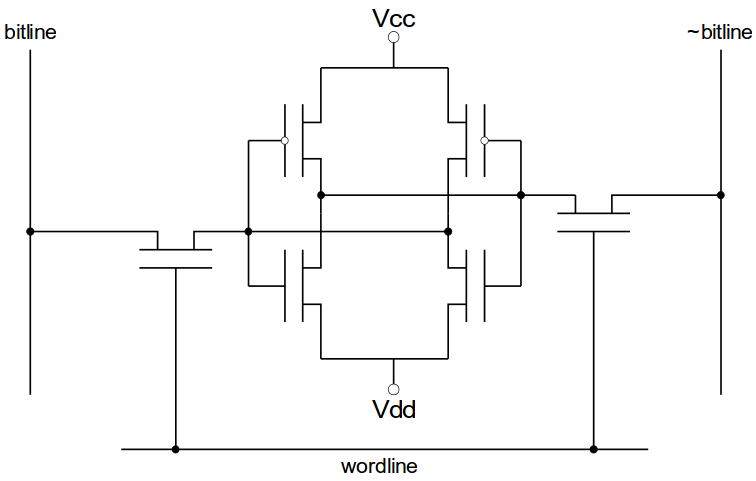
\includegraphics[width=8cm,keepaspectratio=true]{bilder/png/SRAMaufbau}
\caption{Design of a SRAM memory cell\cite{Core16}}
\label{fig:SRAMaufbau}
\end{center}
\end{figure}
\subsubsection{antifuse-based devices}
Antifuse-based devices are OTP. The programming is done with special programming devices. For manufacturing those devices special materials, eg. non-conducting amorphous silicon, are used.\cite{Zeif2011} When antifuse-based devices are programmed, conducting channels are made by high voltage. This can be seen in figure \ref{fig:antifusevorhernachher}. So when antifuse-based FPGAs are programmed the configuration is permanent. This leads to the fact that the configuration of the device is non-volatile and available at power-on. The configuration can be hidden due to special security antifuses. Due to the fact that the device is OTP, no additional memory is needed to store the configuration. The disadvantage of this device is that it can be programmed only once and so it is not suitable for prototyping or changing configurations. Furthermore the programming can only be done off-line.\\
Antifuse-based configurations are radiation hard and therefore suitable for military or space environments.\cite{Maxfield2009} It must be pointed out, that only the configuration is naturally radiation hard, and attached components have to be made radiation hard (shielding, TRD) as well. As antifuses need more manufacturing steps than SRAM-based devices, antifuse-based devices are some technology generations behind.
\begin{figure}[htbp]
\begin{center}
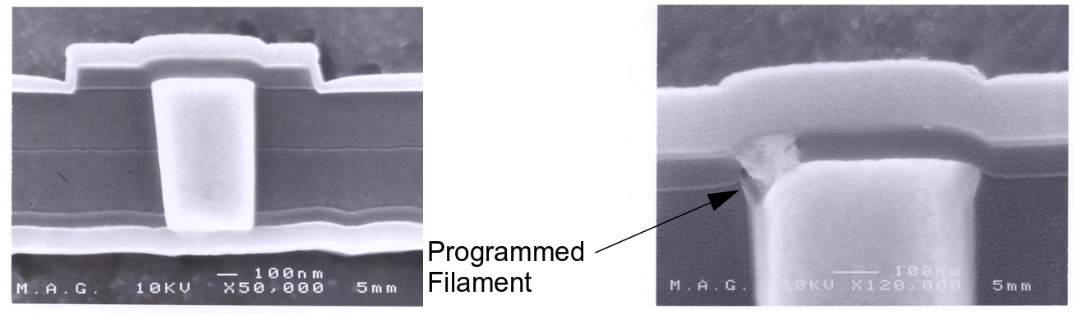
\includegraphics[width=10cm,keepaspectratio=true]{bilder/png/antifusevorhernachher}
\caption{An unprogrammed (left) vs programmed (right) antifuse cell \cite{Qui16}}
\label{fig:antifusevorhernachher}
\end{center}
\end{figure}
\subsubsection{flash-based devices}
\begin{figure}[htbp]
\begin{center}
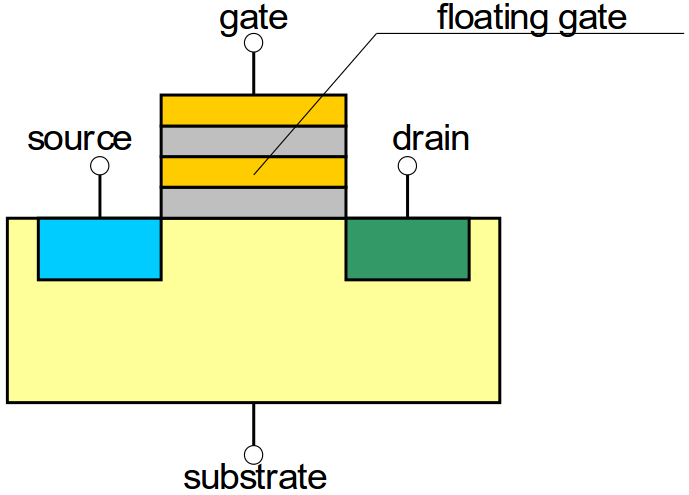
\includegraphics[width=10cm,keepaspectratio=true]{bilder/png/FlashTransistor}
\caption{A floating-gate transistor used in flash memory\cite{Core16}}
\label{fig:FlashTransistor}
\end{center}
\end{figure}
\subsubsection{hybrid systems}
\subsection{System on Chip}
\subsection{Microprocessor system}

\section{Hardware elements}
In this section some important hardware elements are explained.
\subsection{microprocessor}
\begin{figure}[htbp]
\begin{center}
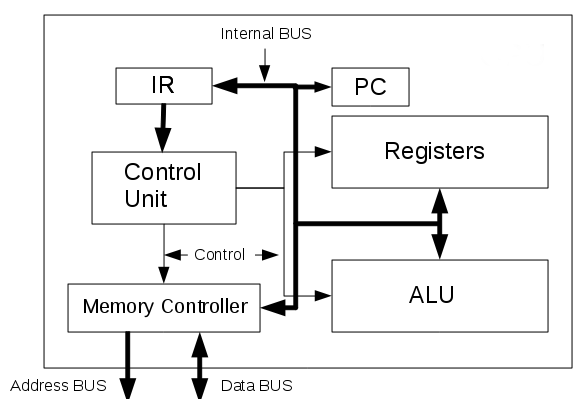
\includegraphics[width=10cm,keepaspectratio=true]{bilder/png/microprocessorblockdiagram}
\caption{Internal structure of a microprocessor}
\label{fig:microprocessorblockdiagram}
\end{center}
\end{figure}
\subsubsection{ARM Cortex A9}
\subsection{flip-flops}
Flipflops are basic logic elements with 2 stable states. They consist of a data input and a clock input, as well as a data output. Optionally a set/reset-pin or an inverted output can be available. Fliipflops are used as memory elements. Simplified, a logical state at the data input is stored at the rising edge of the clock signal, and held stable to the output until the next rising edge occures. The most used flipflop is the D-flipflop.
\begin{itemize}
\item RS-flipflop\\
The RS-flipflop, which can be seen in figure \ref{fig:rsflipflop}, is the most simple form of a flipflop. It consists of a set and a reset input. The state change is asynchrously and therefore not depending on rising clock edges. 

\begin{table}
\begin{center}
\begin{tabular}{|c|c||c|}
\hline
S &  R & $Q_{t+1}$\\
\hline\hline
0 & 0 & $Q_{t}$\\
\hline
0 & 1 & 0\\
\hline
1 & 0 & 1\\
\hline
1 & 1 & undefined\\
\hline
\end{tabular}
\caption{Input/Output states of a RS-flipflop}
\label{tab:rsstates}
\end{center}
\end{table}

The different state transitions of a RS-flipflop are listed in table \ref{tab:rsstates}. As long as the R and S bits are set to low state the output is held constant at the previous state. When the reset bit is set the output is changed to 0, when the set bit is set to 1, Q changes to 1. When R as well as S are both set, the output is simultaneously forced to get low and high. In this metastable state the next state is undefined and is dependent on factoring characterizations.

\begin{figure}[htbp]
\begin{center}
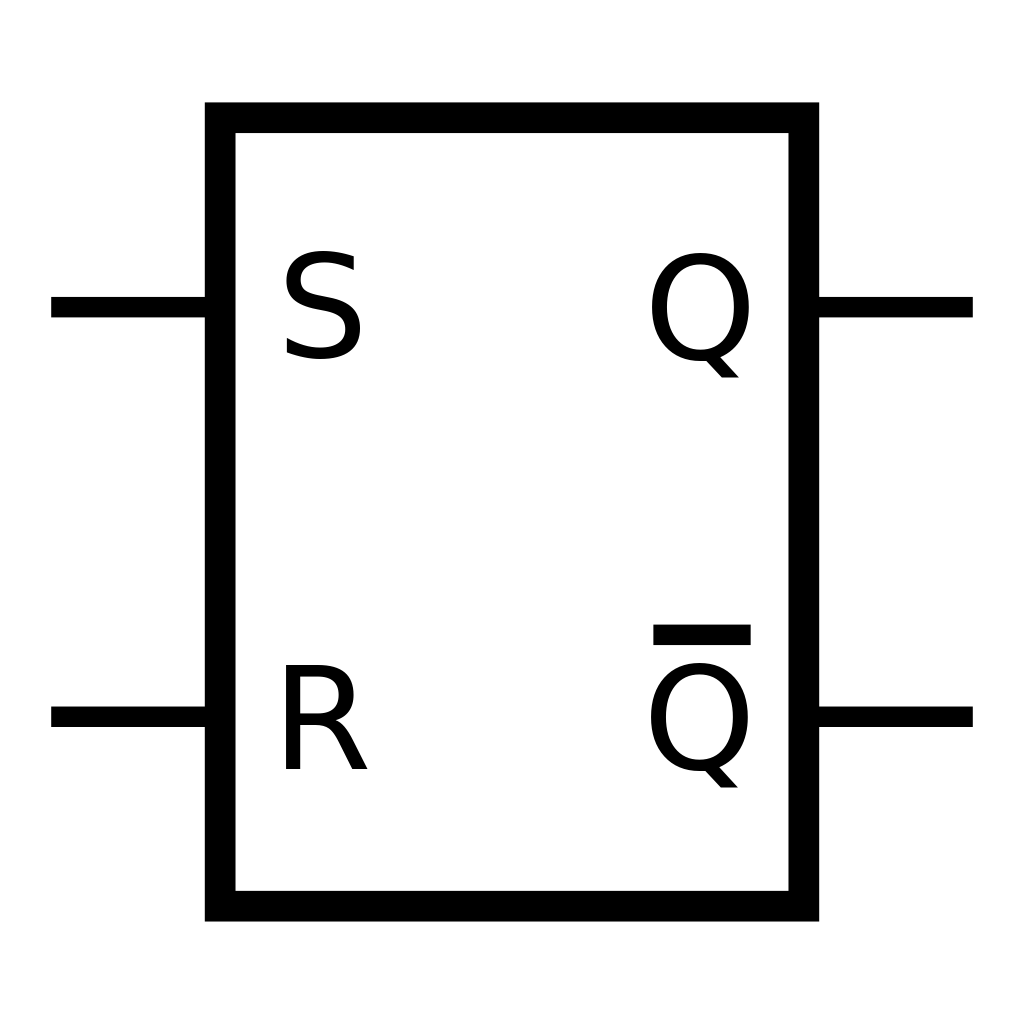
\includegraphics[width=2cm,keepaspectratio=true]{bilder/png/RSflipflop}
\caption{RS-flipflop}
\label{fig:rsflipflop}
\end{center}
\end{figure}
\item RES-flipflop\\
In addition to the simple RS-flipflop this type has an enable input. This causes state changes to only occur when the enable bit is set. The advantage of this configuration is that state changes due to inconsistencies on the input lines. Even though the RES-flipflop has an enable pin it is still an asynchronous device.
\item JK-flipflop\\
The JK-flipflop (shown in figure \ref{fig:jkflipflop} is like a universal flipflop. It can be configured as RS-flipflop D-flipflop as well as a T-flipflop. The state transitions can be found in table \ref{tab:jkstates}. The transitions are like the RS transitions, but as difference the J=K=1 state is interpreted as toggle state.

\begin{table}
\begin{center}
\begin{tabular}{|c|c||c|}
\hline
J &  K & $Q_{t+1}$\\
\hline\hline
0 & 0 & $Q_{t}$\\
\hline
0 & 1 & 0\\
\hline
1 & 0 & 1\\
\hline
1 & 1 & toggle\\
\hline
\end{tabular}
\caption{Input/Output states of a JK-flipflop}
\label{tab:jkstates}
\end{center}
\end{table}
\begin{figure}[htbp]
\begin{center}
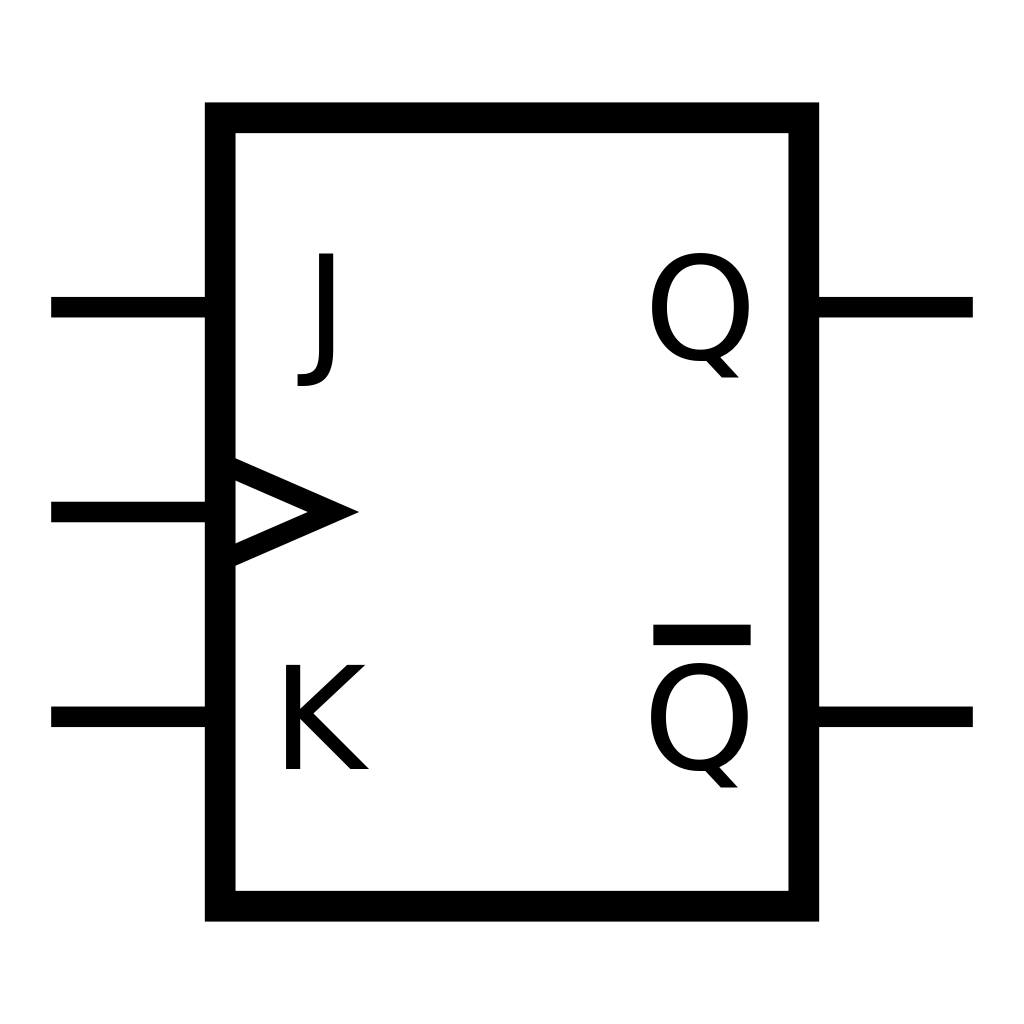
\includegraphics[width=2cm,keepaspectratio=true]{bilder/png/JKflipflop}
\caption{JK-flipflop}
\label{fig:jkflipflop}
\end{center}
\end{figure}
\item T-flipflop\\
The T-flipflop as shown in figure \ref{fig:tflipflop} performs no state transition as long as the T-input is set low. When it is set to 1 the flipflop starts to toggle, the next state will be set to the inverse of the current state, corresponding to the clock rate. The state transitions are listed in table \ref{tab:tstates}.
\begin{table}
\begin{center}
\begin{tabular}{|c||c|}
\hline
T & $Q_{t+1}$\\
\hline\hline
0  & $Q_{t}$\\
\hline
1  & $\overline{Q_{t}}$\\
\hline
\end{tabular}
\caption{Input/Output states of a T-flipflop}
\label{tab:tstates}
\end{center}
\end{table}
\begin{figure}[htbp]
\begin{center}
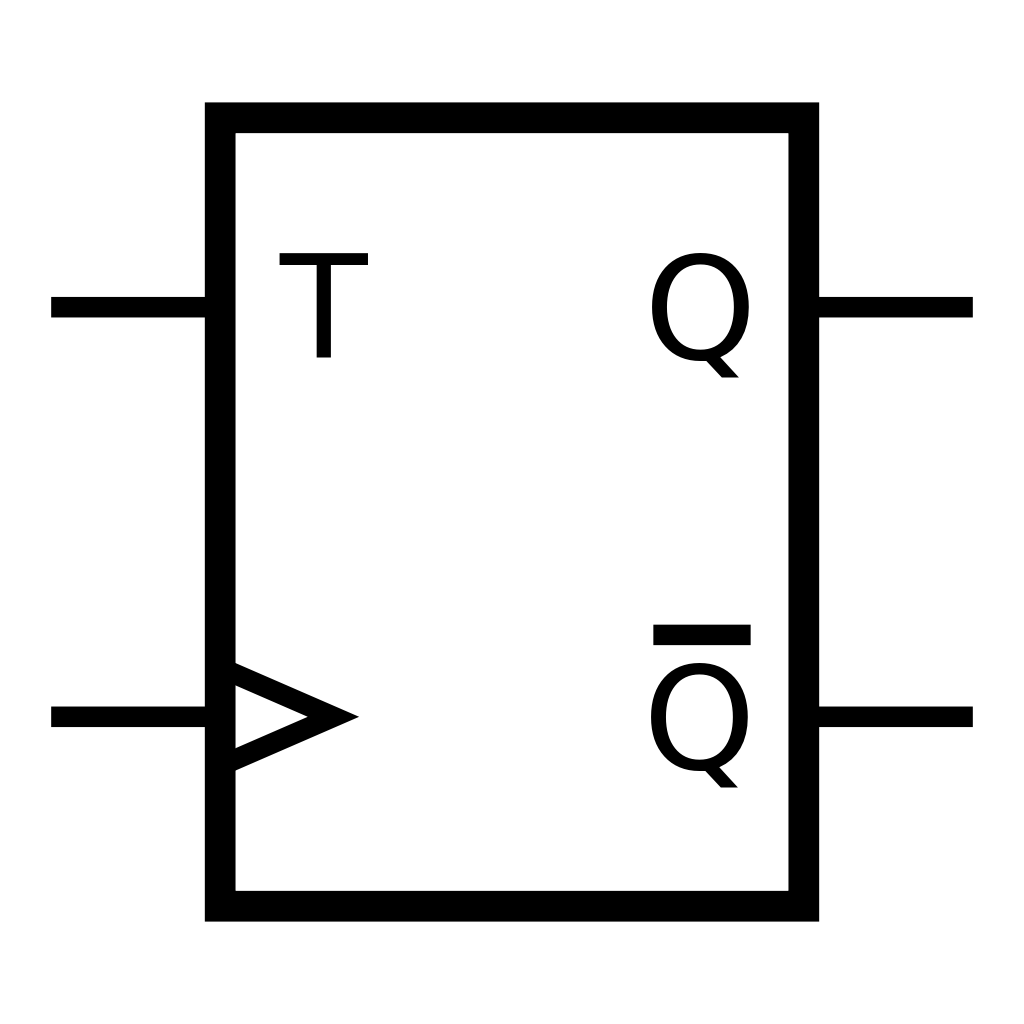
\includegraphics[width=2cm,keepaspectratio=true]{bilder/png/Tflipflop}
\caption{T-flipflop}
\label{fig:tflipflop}
\end{center}
\end{figure}
\item D-flipflop\\
The D-flipflop is the most used flipflop.It can be seen in figure \ref{fig:dflipflop}. The D-flipflop reads the D input at the rising edge of the clock and is therefore a synchronous device. The output is set to the D input at the rising edge and held stable at any other time. In this way the D-flipflop can be seen as simple memory cell
\begin{figure}[htbp]
\begin{center}
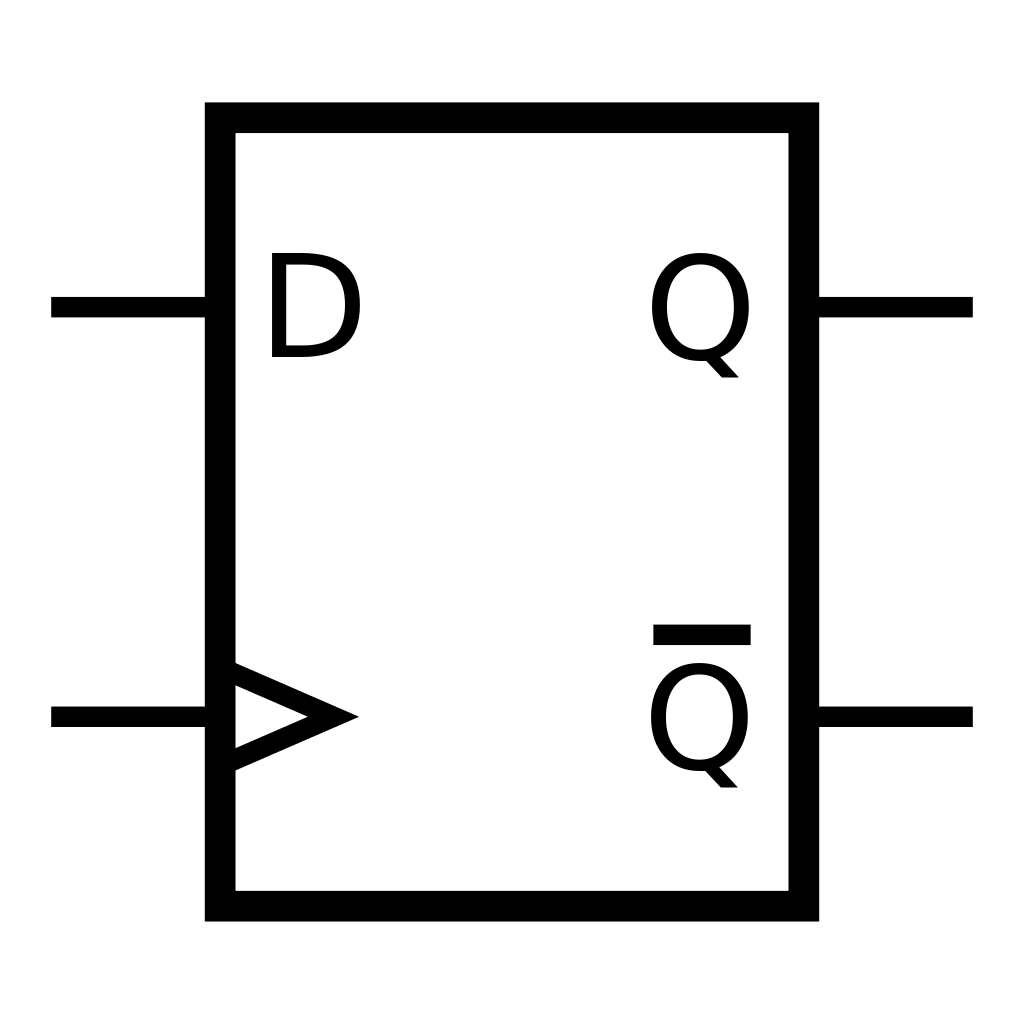
\includegraphics[width=2cm,keepaspectratio=true]{bilder/png/Dflipflop}
\caption{D-flipflop}
\label{fig:dflipflop}
\end{center}
\end{figure}
\end{itemize}
\subsubsection{timing properties}
When using flip-flops some timing parameters are important (seen in figure \ref{fig:flipfloptiming}) and explained below.
\begin{itemize}
\item setup time $t_{S}$\\
The setup time is the time the input signal has to be hold constant before the rising clock of the edge occurs to sample the input reliable, using synchronous devices.
\item hold time $t_{H}$\\
THe hold time is the duration the input signal has to be hold stable after the rising clock edge occured for a reliable input sampling. $t_{H}$ is a property of synchronous flipflops.
\item recovery time\\
The recovery time is like $t_{S}$ for asynchronous flipflops. This is applied, because not every short signal change should have impact on the output. 
\item removal time\\
The removal time is like the hold time for asynchronous devices.
\item propagation delay $t_{P}$, $t_{CO}$\\
The propagation delay is the time the flipflop needs to change the output state after the rising clock edge occured. In some cases the delay times for low-to-high transition is not equal the high-to-low transition time. The propagation delay times are denoted in the datasheets. For correct operation of the flipflop the clock time has to be lower than $t_{S}+t_{H}$.
\end{itemize}
\subsection{memory}

\subsubsection{SDRAM}
\subsubsection{DDR-SDRAM}
\subsection{clock}

\subsubsection{clock signals}
\subsubsection{clock generation}
\paragraph{resonant circuit\\}
The most simple form of generating an oscillating signal is a circuit consisting of a capacitor, inductor and resistor. It oscillates due to the interaction of the magnetic field of the inductor and the electric field of the capacitor. When the capacitor is charged, current flows through the inductor building up a magnetic field. As the capacitor will be decharged the voltage decreases. The magnetic field is a maximum when the capacitor voltage reaches 0. Now the capacitor will start to charge with negative current increasing the electric field while the magnetic field decreases. The circuit starts to oscillate according to Faraday's law. The natural frequency of the oscillation can be determined using
\begin{equation}
f_0=2\pi\omega_0
\end{equation}
with
\begin{equation}
\omega_0=\frac{1}{\sqrt{LC}}
\end{equation}
RLC-circuits are used in many different applications, eg. for tuning radios or as frequency filters. The disadvantages of this type of resonator are the relatively low Q-factor and the fact that resonance frequency is not stable to temperature changes.
\paragraph{crystal oscillator}

\begin{figure}[htbp]
\begin{center}
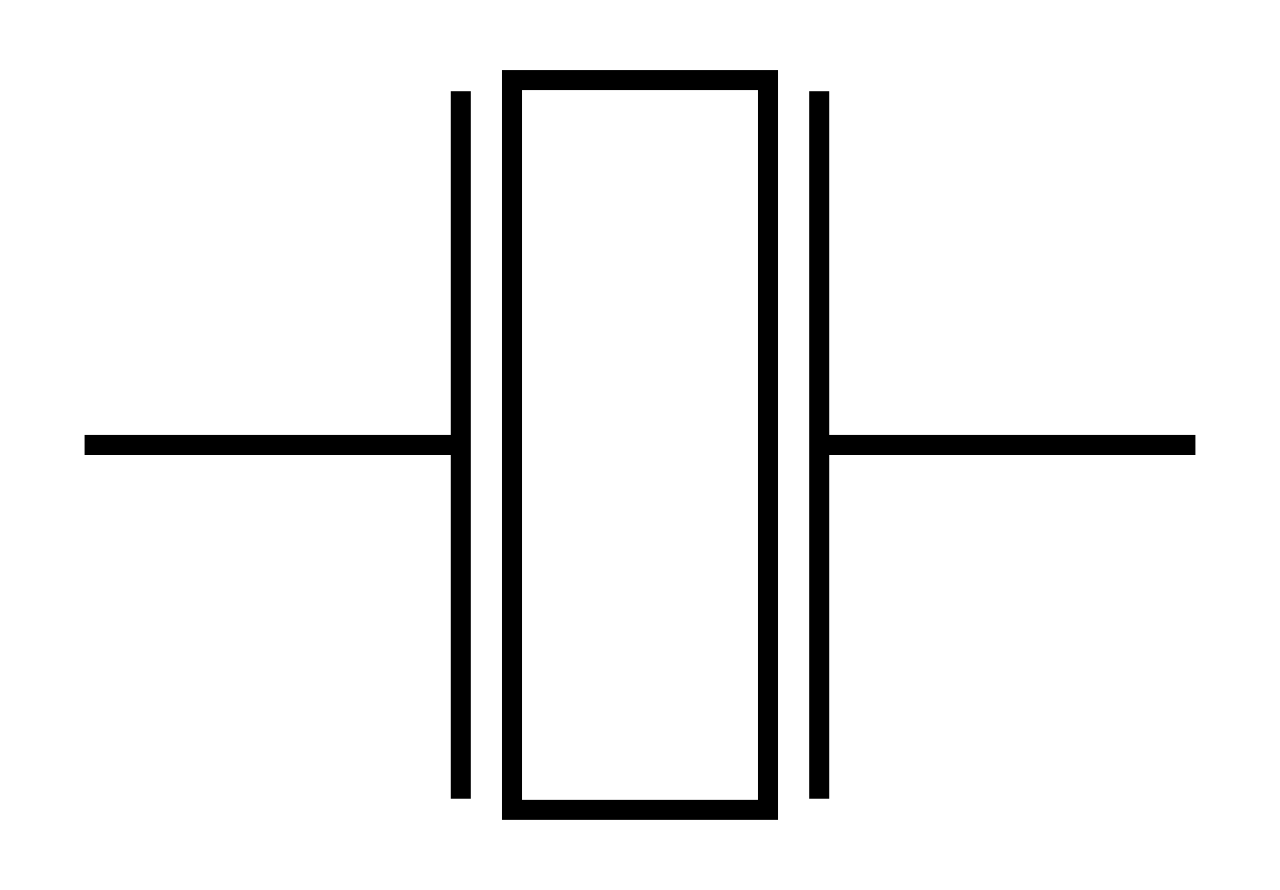
\includegraphics[width=1.5cm,keepaspectratio=true]{bilder/png/crystaloscillatorsymbol}
\caption{IEC symbol of an oscillator}
\label{fig:crystaloscillatorsymbol}
\end{center}
\end{figure}
\paragraph{phase-locked loop}
\begin{figure}[htbp]
\begin{center}
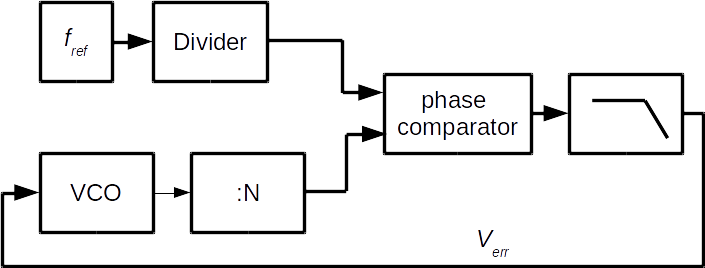
\includegraphics[width=12cm,keepaspectratio=true]{bilder/png/PLLblocks}
\caption{Block diagram of a PLL}
\label{fig:pllblocks}
\end{center}
\end{figure}
\begin{figure}[htbp]
\begin{center}
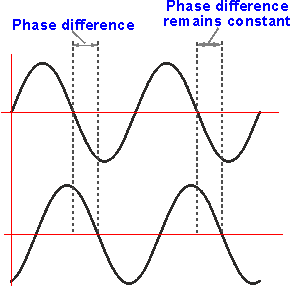
\includegraphics[width=6cm,keepaspectratio=true]{bilder/png/PLLphase}
\caption{Phase diagram of a PLL}
\label{fig:pllphase}
\end{center}
\end{figure}

\subsection{bus technology}

\section{Criticallink MitySOM SoC}
